% =============================================================================
%  Sentinel DV — Conference Presentation Slides (Beamer)
%  DVCon USA / DAC 2026
% =============================================================================
\documentclass[aspectratio=169,t]{beamer}

\usetheme{Madrid}
\usecolortheme{default}

% Custom color scheme (dark blue + teal — Sentinel DV brand)
\definecolor{sdvblue}{RGB}{26,86,219}
\definecolor{sdvdark}{RGB}{17,24,39}
\definecolor{sdvteal}{RGB}{6,148,162}
\definecolor{sdvgreen}{RGB}{5,122,85}
\definecolor{sdvlight}{RGB}{243,244,246}
\definecolor{sdvorange}{RGB}{217,119,6}
\definecolor{sdvred}{RGB}{224,36,36}

\setbeamercolor{palette primary}{bg=sdvblue,fg=white}
\setbeamercolor{palette secondary}{bg=sdvdark,fg=white}
\setbeamercolor{palette tertiary}{bg=sdvteal,fg=white}
\setbeamercolor{palette quaternary}{bg=sdvdark,fg=white}
\setbeamercolor{structure}{fg=sdvblue}
\setbeamercolor{section in toc}{fg=sdvdark}
\setbeamercolor{block title}{bg=sdvblue,fg=white}
\setbeamercolor{block body}{bg=sdvlight,fg=sdvdark}
\setbeamercolor{alertblock title}{bg=sdvred,fg=white}
\setbeamercolor{alertblock body}{bg=sdvlight,fg=sdvdark}
\setbeamercolor{exampleblock title}{bg=sdvgreen,fg=white}
\setbeamercolor{exampleblock body}{bg=sdvlight,fg=sdvdark}

\usepackage[T1]{fontenc}
\usepackage[utf8]{inputenc}
\usepackage{graphicx}
\usepackage{booktabs}
\usepackage{listings}
\usepackage{xcolor}
\usepackage{tikz}

\usepackage{microtype}
\usepackage{array}
\usepackage{colortbl}

\lstdefinestyle{mcp}{
  backgroundcolor=\color{sdvdark},
  basicstyle=\ttfamily\small\color{white},
  keywordstyle=\color{sdvteal}\bfseries,
  stringstyle=\color{sdvgreen},
  commentstyle=\color{gray}\itshape,
  breaklines=true,
  frame=none,
  numbers=none,
}

\setbeamertemplate{navigation symbols}{}
\setbeamertemplate{footline}[frame number]

\title[Sentinel DV — DVCon/DAC 2026]{%
  \textbf{Sentinel DV}\\[4pt]
  \large An Open-Source MCP Server for\\
  AI-Assisted Design Verification Intelligence
}
\subtitle{DVCon USA / DAC 2026}
\author{Open-Source Contribution}
\institute{\textbf{[GitHub]}\ \texttt{github.com/kiranreddi/sentinel-dv} \quad MIT License}
\date{2026}

% =============================================================================
\begin{document}

% ---- Title Slide ----
\setbeamercolor{background canvas}{bg=sdvdark}
\setbeamercolor{title}{fg=white}
\setbeamercolor{subtitle}{fg=sdvteal}
\setbeamercolor{author}{fg=white}
\setbeamercolor{institute}{fg=sdvlight}
\setbeamercolor{date}{fg=sdvlight}
\begin{frame}[plain]
  \titlepage
  \vspace{-1em}
  \begin{center}
    \small\color{sdvlight}
    \textbf{26 MCP Tools} \quad|\quad
    \textbf{3 Simulator Vendors} \quad|\quad
    \textbf{1,477 CI Runs Validated} \quad|\quad
    \textbf{Open Source (MIT)}
  \end{center}
\end{frame}
\setbeamercolor{background canvas}{bg=white}

% ---- Outline ----
\begin{frame}{Agenda}
  \tableofcontents
\end{frame}

% =============================================================================
\section{The Problem}
\begin{frame}{The DV Toolchain Fragmentation Problem}
  \begin{columns}[T]
    \column{0.48\textwidth}
      \begin{alertblock}{What DV Engineers Face Today}
        \begin{itemize}
          \item \textbf{10,000s} of simulation logs — no unified query
          \item Coverage databases locked in proprietary formats
          \item Failures scattered across VCS, Questa, Xcelium
          \item Manual log triage takes \textbf{hours per regression}
          \item AI assistants have \textbf{no interface} to sim artifacts
        \end{itemize}
      \end{alertblock}
      \vspace{0.5em}
      \begin{block}{The Opportunity}
        LLMs (Claude, GPT-4, Copilot) can reason deeply over structured
        data — but only if they can \emph{access} it.
      \end{block}

    \column{0.48\textwidth}
      \begin{exampleblock}{Typical DV Artifact Silos}
        \vspace{0.3em}
        \begin{tabular}{ll}
          \textbf{Format}      & \textbf{Viewer} \\
          \hline
          UVM logs (.log)      & grep / Perl \\
          VDB / UCDB           & Verdi / Questa \\
          Assertion JSON       & manual parse \\
          JUnit XML            & Jenkins only \\
          VCD waveforms        & GTKWave \\
          Regression logs      & spreadsheet \\
        \end{tabular}
        \vspace{0.3em}\\
        \textit{None of these expose a query API suitable for AI.}
      \end{exampleblock}
  \end{columns}
\end{frame}

% =============================================================================
\section{Model Context Protocol}
\begin{frame}[fragile]{Model Context Protocol (MCP)}
  \begin{columns}[T]
    \column{0.55\textwidth}
      \begin{block}{What is MCP?}
        \begin{itemize}
          \item Open standard by Anthropic (Nov 2024)
          \item JSON-RPC 2.0 over stdio or SSE
          \item AI \textbf{client} discovers and calls \textbf{tools}
                exposed by a \textbf{server}
          \item Adopted by Claude, GPT-4o, Copilot, Cursor
          \item Zero code changes to the AI — just plug in the server
        \end{itemize}
      \end{block}

      \vspace{0.5em}
      \begin{exampleblock}{MCP Tool Call (JSON-RPC)}
\begin{semiverbatim}\color{white}
{
  "method": "tools/call",
  "params": {
    "name": "regression.health",
    "arguments": {}
  }
}
\end{semiverbatim}
      \end{exampleblock}

    \column{0.40\textwidth}
      \begin{block}{Why MCP for DV?}
        \begin{itemize}
          \item Sim artifacts $\rightarrow$ structured tools
          \item AI reasons over \emph{your} regression
          \item Works with any LLM that supports MCP
          \item Runs in CI — no GUI required
          \item Output schemas validated (Pydantic)
          \item Path redaction built in
        \end{itemize}
      \end{block}
  \end{columns}
\end{frame}

% =============================================================================
\section{Sentinel DV Architecture}
\begin{frame}{Sentinel DV — System Architecture}
  \begin{center}
    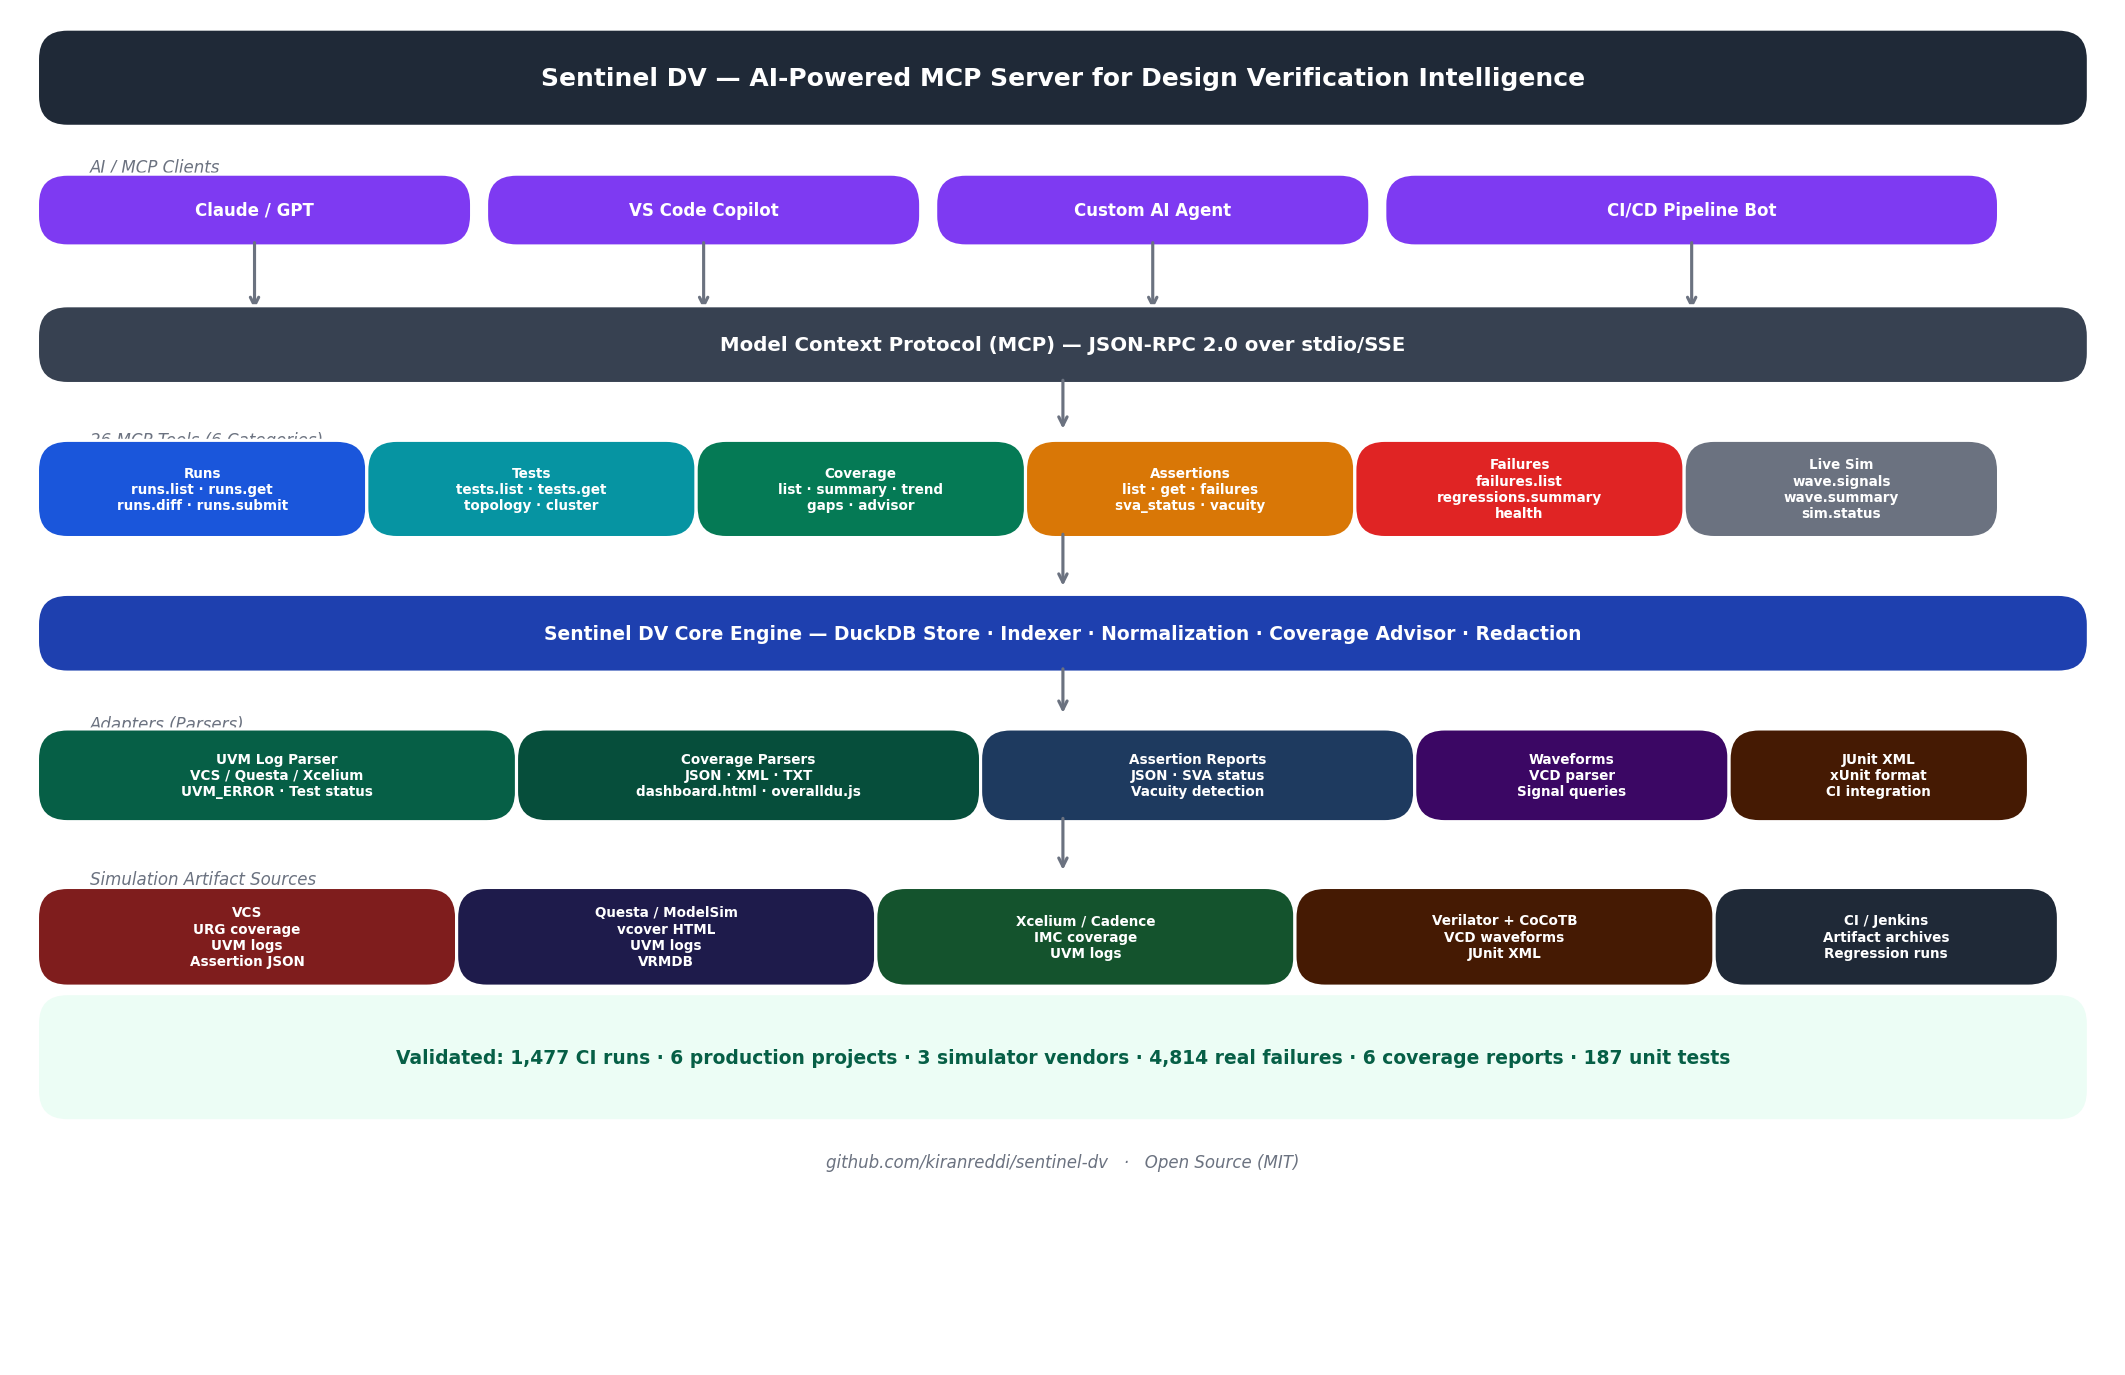
\includegraphics[width=0.92\textwidth]{../figures/architecture.png}
  \end{center}
\end{frame}

% =============================================================================
\section{26 MCP Tools}
\begin{frame}{26 MCP Tools — Six Categories}
  \begin{columns}[T]
    \column{0.32\textwidth}
      \begin{block}{Chart\ Run Tracking (4)}
        \texttt{runs.list} · \texttt{runs.get}\\
        \texttt{runs.diff} · \texttt{runs.submit}\\
        \texttt{runs.cross\_sim}
      \end{block}
      \vspace{0.3em}
      \begin{block}{Test\ Test Analysis (5)}
        \texttt{tests.list} · \texttt{tests.get}\\
        \texttt{tests.topology}\\
        \texttt{tests.replay} · \texttt{tests.cluster}
      \end{block}
      \vspace{0.3em}
      \begin{block}{Assert\ Assertion Engine (5)}
        \texttt{assertions.list} · \texttt{.get}\\
        \texttt{.failures} · \texttt{.sva\_status}\\
        \texttt{.vacuity}
      \end{block}

    \column{0.32\textwidth}
      \begin{block}{Cov\ Coverage Intel. (5)}
        \texttt{coverage.list} · \texttt{.summary}\\
        \texttt{.trend} · \texttt{.gaps}\\
        \texttt{.advisor}
      \end{block}
      \vspace{0.3em}
      \begin{block}{Bug\ Failure Triage (4)}
        \texttt{failures.list}\\
        \texttt{regressions.summary}\\
        \texttt{regression.health}
      \end{block}
      \vspace{0.3em}
      \begin{block}{Wave\ Live Sim (3)}
        \texttt{wave.signals}\\
        \texttt{wave.summary}\\
        \texttt{sim.status}
      \end{block}

    \column{0.32\textwidth}
      \begin{alertblock}{*\ 5 DV Intelligence Tools}
        \vspace{0.2em}
        \small
        \textbf{coverage.trend}\\
        Time-series trajectory + direction\\[4pt]
        \textbf{runs.cross\_sim}\\
        Cross-vendor divergence\\[4pt]
        \textbf{tests.cluster}\\
        Root-cause grouping\\[4pt]
        \textbf{regression.health}\\
        0--100 DV readiness score\\[4pt]
        \textbf{coverage.advisor}\\
        SV constraint generation
      \end{alertblock}
  \end{columns}
\end{frame}

% =============================================================================
\begin{frame}[fragile]{Multi-Simulator UVM Log Parsing}
  \begin{columns}[T]
    \column{0.48\textwidth}
      \begin{block}{Three Simulator Formats Supported}
        \begin{tabular}{ll}
          \toprule
          \textbf{Simulator} & \textbf{Format Prefix} \\
          \midrule
          VCS (Synopsys) & \texttt{UVM\_ERROR file(line) @} \\
          Questa (Siemens) & \texttt{\# UVM\_ERROR @ time} \\
          Xcelium (Cadence) & \texttt{xcelium: UVM\_ERROR} \\
          \bottomrule
        \end{tabular}
      \end{block}
      \vspace{0.4em}
      \begin{alertblock}{Critical Fix: Count-Summary Lines}
        \small
        VCS logs end with \texttt{UVM\_ERROR :\ \ \ 0}\\
        Naive regex creates \textbf{16,240} false failures!\\[4pt]
        \textbf{UVM\_COUNT\_SUMMARY\_PATTERN} skips these:\\
        Result: \textbf{4,380 real failures} (73\% reduction)
      \end{alertblock}

    \column{0.48\textwidth}
      \begin{exampleblock}{Parser in Action — VCS Log}
\begin{semiverbatim}\color{white}
UVM_ERROR scbd.sv(88) @ 500ns:
  env.scbd [MISMATCH]
  Expected 0xDEAD got 0xBEEF

--- UVM Report Summary ---
UVM_ERROR :    1   <- parsed
UVM_ERROR :    0   <- SKIPPED
\end{semiverbatim}
      \end{exampleblock}
      \vspace{0.3em}
      \begin{exampleblock}{MCP Tool Result}
\begin{semiverbatim}\color{white}
failures.list -> {
  "message": "[MISMATCH] Expected
    0xDEAD got 0xBEEF",
  "category": "data_mismatch",
  "severity": "UVM_ERROR"
}
\end{semiverbatim}
      \end{exampleblock}
  \end{columns}
\end{frame}

% =============================================================================
\section{Coverage Intelligence}
\begin{frame}[fragile]{Coverage HTML Parsers — No DB Access Needed}
  \begin{columns}[T]
    \column{0.48\textwidth}
      \begin{block}{VCS URG \texttt{dashboard.html}}
        \begin{itemize}
          \item Generated by \texttt{urg -report}
          \item Content-sniff: ``Total Coverage Summary''
          \item Extracts: SCORE, LINE, TOGGLE, ASSERT, GROUP
          \item \textbf{+ Verification Plan score}
          \item Zero access to \texttt{simv.vdb} needed
        \end{itemize}
      \end{block}
      \vspace{0.3em}
      \begin{block}{Questa vcover \texttt{overalldu.js}}
        \begin{itemize}
          \item Generated by \texttt{vcover report -html}
          \item Single-line JS file (regex fails!)
          \item \textbf{Balanced-brace JSON scanner}
          \item Extracts: stmt, branch, toggle, assert,\\
                functional, total + hit/total counts
        \end{itemize}
      \end{block}

    \column{0.48\textwidth}
      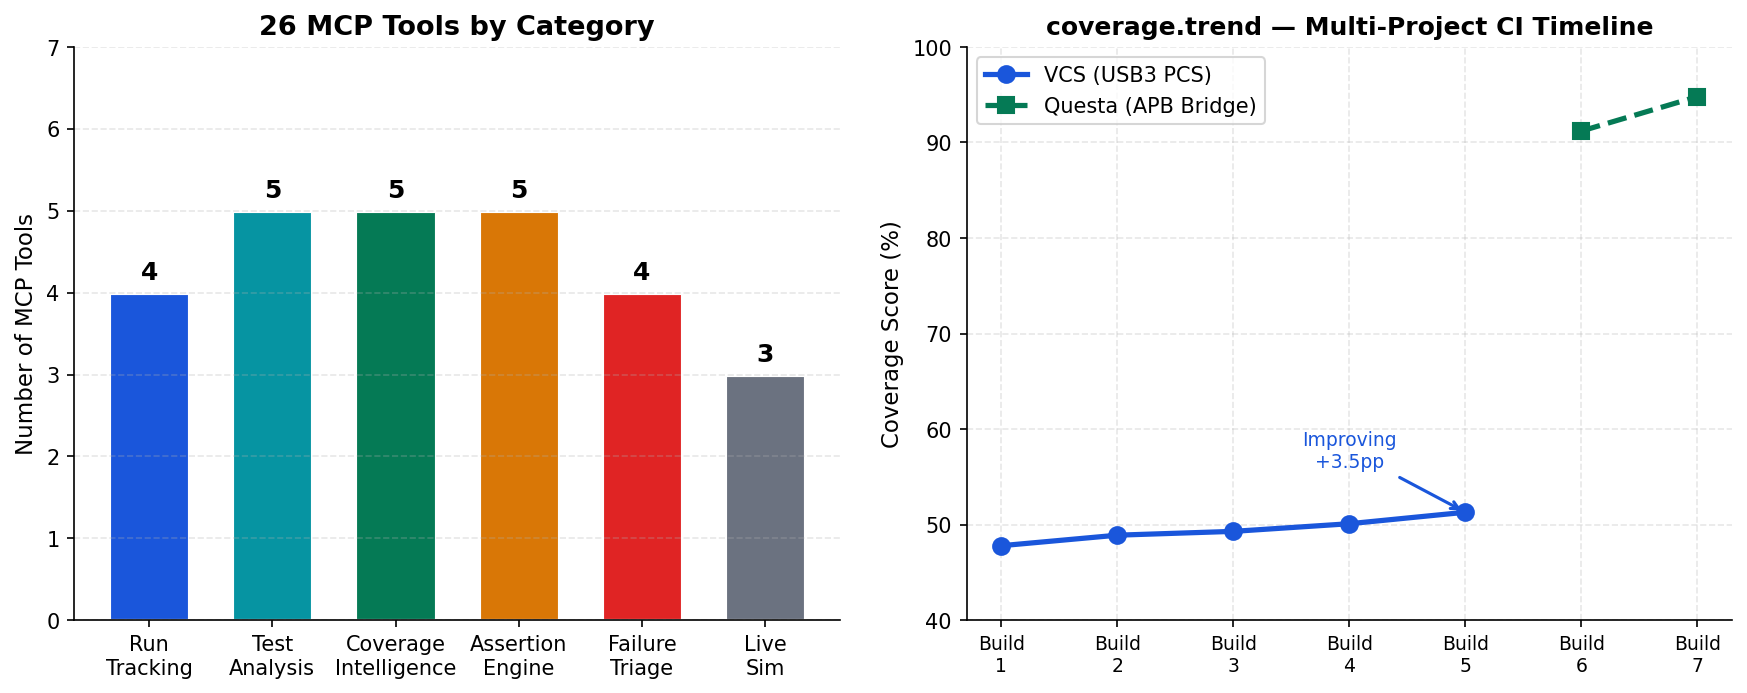
\includegraphics[width=\textwidth]{../figures/tools_coverage.png}
      \vspace{0.2em}
      \begin{exampleblock}{coverage.summary output}
\begin{semiverbatim}\color{white}
{
  "summaries": [{
    "kind": "code",
    "metrics": [
      {"name":"line",    "covered":87.3},
      {"name":"toggle",  "covered":62.1},
      {"name":"branch",  "covered":71.5},
      {"name":"assertion","covered":100.0}
    ]
  }]
}
\end{semiverbatim}
      \end{exampleblock}
  \end{columns}
\end{frame}

% =============================================================================
\begin{frame}[fragile]{DV Intelligence — Regression Health Score}
  \begin{columns}[T]
    \column{0.52\textwidth}
      \begin{block}{Composite Health Formula}
        \[
          H = 0.30 P + 0.35 C + 0.15 A + 0.10 F + 0.10 X
        \]
        \vspace{-0.5em}
        \begin{itemize}
          \item $P$ = pass rate (30\% weight)
          \item $C$ = coverage score (35\% weight)
          \item $A$ = assertion health (15\% weight)
          \item $F$ = flakiness inverse (10\% weight)
          \item $X$ = cross-sim consistency (10\% weight)
        \end{itemize}
      \end{block}
      \vspace{0.3em}
      \begin{block}{Bands}
        \begin{tabular}{ll}
          $H \geq 90$ & \textcolor{sdvgreen}{\textbf{sign-off-ready}} \\
          $H \geq 75$ & \textcolor{sdvblue}{\textbf{minor-issues}} \\
          $H \geq 55$ & \textcolor{sdvorange}{\textbf{coverage-gaps}} \\
          $H < 55$    & \textcolor{sdvred}{\textbf{not-ready}} \\
        \end{tabular}
      \end{block}

    \column{0.44\textwidth}
      \begin{exampleblock}{Example Output}
\begin{semiverbatim}\color{white}
regression.health -> {
  "health_score": 77.5,
  "band": "minor-issues",
  "grade": "B+",
  "components": {
    "pass_rate":    94.2,
    "coverage":     51.3,
    "assertions":   100.0,
    "flakiness":    98.1,
    "cross_sim":    87.5
  },
  "recommendations": [
    "Coverage below target (51%)",
    "3 tests flaky across sims"
  ]
}
\end{semiverbatim}
      \end{exampleblock}
  \end{columns}
\end{frame}

% =============================================================================
\begin{frame}[fragile]{DV Intelligence — Coverage Advisor}
  \begin{columns}[T]
    \column{0.50\textwidth}
      \begin{block}{What it Does}
        \begin{itemize}
          \item Finds coverage gaps $<$ threshold (default 25\%)
          \item Detects protocol from signal names:\\
                AXI4, AHB, APB, CHI, PCIe, USB
          \item Generates \textbf{ready-to-paste} SystemVerilog\\
                constraints and UVM sequences
          \item Prioritized: \texttt{high} / \texttt{medium} / \texttt{low}
        \end{itemize}
      \end{block}
      \vspace{0.3em}
      \begin{alertblock}{AI + Advisor = Instant Fix}
        \small
        Engineer: \textit{"How do I close the WRAP burst coverage?"}\\[4pt]
        AI calls \texttt{coverage.advisor} and replies:\\
        \textit{"Add this constraint to your AXI4 driver:\ldots"}\\
        \small\texttt{awburst inside \{INCR, WRAP, FIXED\};}
      \end{alertblock}

    \column{0.46\textwidth}
      \begin{exampleblock}{coverage.advisor JSON Output}
\begin{semiverbatim}\color{white}
{
  "priority": "high",
  "kind": "toggle",
  "gap_pct": 18.3,
  "recommendation":
    "Uncovered: AXI4 AWBURST signal",
  "sv_constraint":
    "constraint c_burst {\n"
    "  awburst inside "
    "{INCR, WRAP};\n}",
  "uvm_sequence":
    "// Drive WRAP burst\n"
    "tx.burst_type = WRAP;\n"
    "tx.len = $urandom_range(1,15);"
}
\end{semiverbatim}
      \end{exampleblock}
  \end{columns}
\end{frame}

% =============================================================================
\section{AXI4 Demo \& Validation}
\begin{frame}[fragile]{AXI4 UVM 3-Simulator Demo}
  \begin{columns}[T]
    \column{0.50\textwidth}
      \begin{block}{What's in the Demo}
        \begin{itemize}
          \item \texttt{demo/axi4\_uvm/} in the repository
          \item AXI4-Lite slave DUT + UVM testbench
          \item 4 tests: back-to-back, error resp, boundary, stress
          \item Pre-generated artifacts for \textbf{all 3 simulators}:
                VCS, Questa, Xcelium
          \item Results, assertions, coverage, waveforms per sim
          \item \textbf{5 seconds} to index + run all 26 tools
        \end{itemize}
      \end{block}
      \vspace{0.3em}
      \begin{block}{Demo Structure}
        \small
        \texttt{demo/axi4\_uvm/vcs/} \\
        \texttt{demo/axi4\_uvm/questa/} \\
        \texttt{demo/axi4\_uvm/xcelium/} \\
        Each: results.xml, assertions/*.json,\\
        coverage/*.json, waveforms/*.wave.json
      \end{block}

    \column{0.46\textwidth}
      \begin{exampleblock}{runs.cross\_sim — Divergence}
\begin{semiverbatim}\color{white}
runs.cross_sim -> {
  "simulators_compared": 3,
  "divergent_tests": [
    {
      "test": "axi4_stress_test",
      "vcs": "pass",
      "questa": "fail",
      "xcelium": "pass",
      "critical": true
    }
  ]
}
\end{semiverbatim}
      \end{exampleblock}
      \vspace{0.2em}
      \begin{exampleblock}{tests.cluster — Root Causes}
\begin{semiverbatim}\color{white}
tests.cluster -> {
  "clusters": [
    {
      "size": 3,
      "category": "timeout",
      "representative":
        "[TIMEOUT] WRAP burst test"
    }
  ]
}
\end{semiverbatim}
      \end{exampleblock}
  \end{columns}
\end{frame}

% =============================================================================
\section{Evaluation Results}
\begin{frame}{Validation Results — 1,477 Real CI Runs}
  \begin{columns}[T]
    \column{0.50\textwidth}
      \begin{center}
        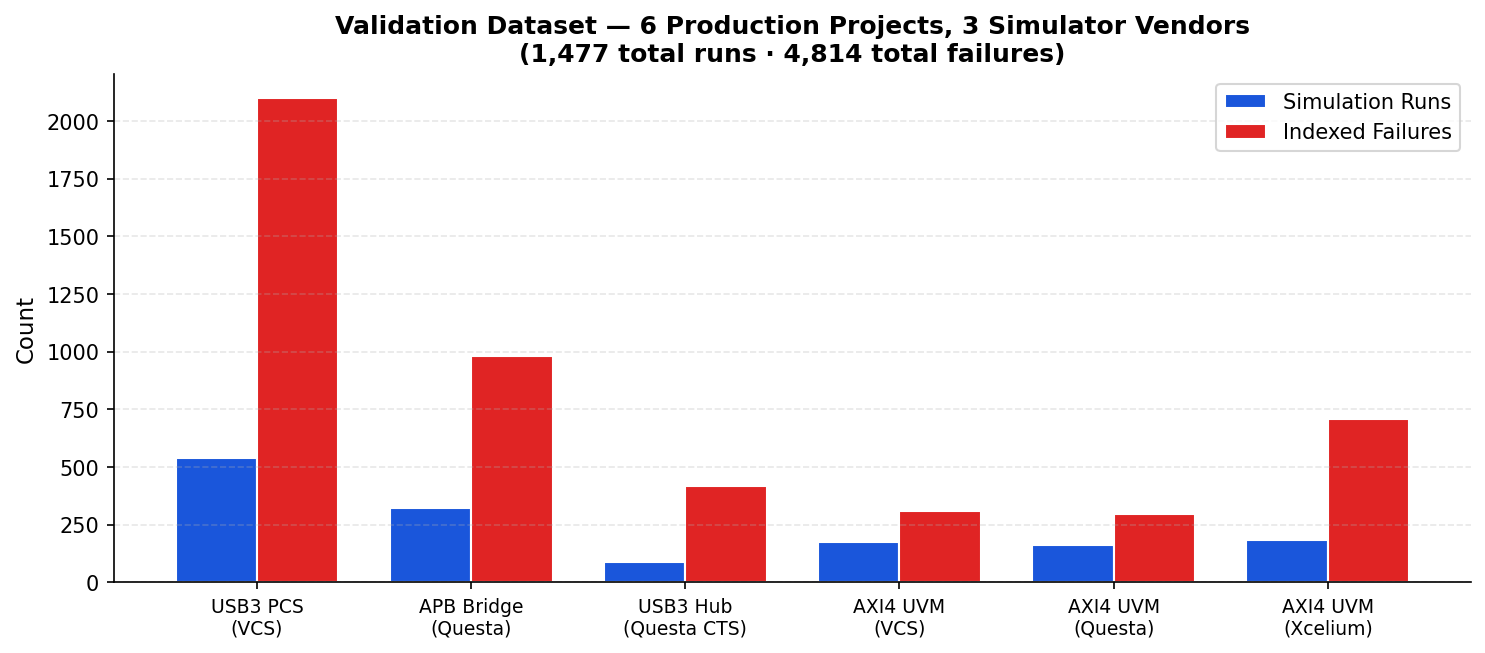
\includegraphics[width=\textwidth]{../figures/validation_results.png}
      \end{center}

    \column{0.46\textwidth}
      \begin{block}{Dataset Summary}
        \begin{tabular}{lr}
          \toprule
          \textbf{Metric} & \textbf{Value} \\
          \midrule
          Total CI runs indexed   & 1,477 \\
          Total tests             & 2,611 \\
          Total failures          & 4,814 \\
          Coverage reports        & 6 \\
          Projects                & 6 \\
          Simulator vendors       & 3 \\
          Unit tests              & 187 \\
          \bottomrule
        \end{tabular}
      \end{block}
      \vspace{0.3em}
      \begin{exampleblock}{Tool Validation}
        \begin{tabular}{lr}
          \textbf{PASS} (live data)  & \textbf{20/26} \\
          \textbf{SKIP} (needs sim)  & 5/26 \\
          \textbf{SKIP} (no dataset) & 1/26 \\
          \textbf{FAIL}              & \textbf{0/26} \\
        \end{tabular}
      \end{exampleblock}
      \vspace{0.2em}
      \small\textcolor{sdvgreen}{\textbf{Zero tool failures on real production data.}}
  \end{columns}
\end{frame}

% =============================================================================
\section{AI Session Demo}
\begin{frame}[fragile]{Real AI Session with Sentinel DV}
  \begin{columns}[T]
    \column{0.50\textwidth}
      \begin{block}{Engineer Asks}
        \large\textit{``What's wrong with today's regression?\\
        How do I close coverage?''}
      \end{block}
      \vspace{0.3em}
      \small
      \textbf{AI calls in sequence:}
      \begin{enumerate}
        \item \texttt{regression.health} — gets overall score
        \item \texttt{tests.cluster} — groups 18 timeout failures
        \item \texttt{coverage.gaps} — finds WRAP burst uncovered
        \item \texttt{coverage.advisor} — generates SV constraint
      \end{enumerate}
      \vspace{0.3em}
      \begin{alertblock}{AI Response (30 seconds)}
        \small
        ``18 tests time out on AXI4 WRAP burst — health
        score is 62 (coverage-gaps band). Add:
        \texttt{awburst inside \{INCR,WRAP\};} to your
        driver. 6 more tests have AWVALID assertion
        failures — fix the burst timeout first.''
      \end{alertblock}

    \column{0.46\textwidth}
\begin{semiverbatim}\color{white}
# regression.health
health_score: 62.1
band: "coverage-gaps"

# tests.cluster
clusters:
  - size: 18
    category: timeout
    rep: "[TIMEOUT] WRAP burst"
  - size: 6
    category: assertion
    rep: "[ASSERT] AWVALID"

# coverage.gaps
gaps:
  - kind: "toggle"
    gap_pct: 48.7
    scope: "axi4_master.AWBURST"

# coverage.advisor
advisories:
  - priority: "high"
    sv_constraint: |
      constraint c_burst {
        awburst inside
          {INCR, WRAP};
      }
\end{semiverbatim}
  \end{columns}
\end{frame}

% =============================================================================
\section{Getting Started}
\begin{frame}[fragile]{Installation \& Quick Start}
  \begin{columns}[T]
    \column{0.48\textwidth}
      \begin{block}{Install}
\begin{semiverbatim}\color{white}
pip install sentinel-dv
\end{semiverbatim}
      \end{block}
      \vspace{0.3em}
      \begin{block}{Configure (\texttt{sentinel\_dv.yaml})}
\begin{semiverbatim}\color{white}
artifact_roots:
  - /path/to/sim/logs
  - /path/to/coverage/report
  - /path/to/coverage/files

db_path: ./sentinel_dv.db
\end{semiverbatim}
      \end{block}
      \vspace{0.3em}
      \begin{block}{Run Server}
\begin{semiverbatim}\color{white}
sentinel-dv serve \
  --config sentinel_dv.yaml
\end{semiverbatim}
      \end{block}

    \column{0.48\textwidth}
      \begin{block}{Add to Claude / VS Code MCP Config}
\begin{semiverbatim}\color{white}
{
  "mcpServers": {
    "sentinel-dv": {
      "command": "sentinel-dv",
      "args": ["serve",
        "--config", "sentinel_dv.yaml"]
    }
  }
}
\end{semiverbatim}
      \end{block}
      \vspace{0.3em}
      \begin{exampleblock}{Try the AXI4 Demo}
\begin{semiverbatim}\color{white}
git clone github.com/kiranreddi/
  sentinel-dv
cd sentinel-dv
sentinel-dv index \
  --config demo/axi4_uvm/config.yaml
# Then connect your AI assistant!
\end{semiverbatim}
      \end{exampleblock}
  \end{columns}
\end{frame}

% =============================================================================
\section{Conclusion}
\begin{frame}{Conclusion \& Future Work}
  \begin{columns}[T]
    \column{0.50\textwidth}
      \begin{block}{What We Built}
        \begin{itemize}
          \item \textbf{26 MCP tools} — full DV workflow coverage
          \item \textbf{3-simulator} UVM log parsing (zero false positives)
          \item \textbf{HTML coverage parsers} — no DB access needed
          \item \textbf{5 DV intelligence tools} — trend, clustering,
                health score, advisor
          \item Validated on \textbf{1,477 real CI runs}, 6 projects
          \item \textbf{187 unit tests}, all green
          \item \textbf{CI green} on GitHub Actions (Python 3.10/3.11/3.12)
        \end{itemize}
      \end{block}

    \column{0.46\textwidth}
      \begin{alertblock}{Future Work}
        \begin{itemize}
          \item FSDB/MXDB waveform parsing
          \item Direct UCDB/VDB parsing (no export)
          \item Formal property synthesis from coverage gaps
          \item Cloud MCP endpoint for CI/CD
          \item Test generation from failure clusters
          \item Coverage-aware testplan tracking
        \end{itemize}
      \end{alertblock}
      \vspace{0.5em}
      \begin{center}
        \Large\textbf{[GitHub]}\ \texttt{kiranreddi/sentinel-dv}\\[4pt]
        \normalsize MIT License · PyPI: \texttt{pip install sentinel-dv}\\[4pt]
        \textcolor{sdvgreen}{\textbf{Stars *\ Welcome!}}
      \end{center}
  \end{columns}
\end{frame}

% ---- Thank You ----
\setbeamercolor{background canvas}{bg=sdvdark}
\begin{frame}[plain]
  \begin{center}
    \vspace{1.5em}
    {\Huge\color{white}\textbf{Thank You}}\\[1em]
    {\large\color{sdvteal} Questions?}\\[2em]
    {\large\color{white}
      \textbf{[GitHub]}\ \texttt{github.com/kiranreddi/sentinel-dv}\\[0.5em]
      \texttt{pip install sentinel-dv}
    }\\[2em]
    \begin{tabular}{ccc}
      \textcolor{white}{\textbf{26 MCP Tools}} &
      \textcolor{white}{\textbf{3 Simulators}} &
      \textcolor{white}{\textbf{1,477 CI Runs}} \\
      \textcolor{sdvteal}{Full DV Workflow} &
      \textcolor{sdvteal}{VCS·Questa·Xcelium} &
      \textcolor{sdvteal}{Production Validated} \\
    \end{tabular}
  \end{center}
\end{frame}

\end{document}
